\section{Testing plan}

The main goals of this performance testing plan are:
\begin{itemize}
  \item to find out whether the usage of LSM implies some sort of performance penalty;
  \item to identify possible improvements when embedding WebAssembly in another language.
\end{itemize}

\noindent
For a given program written in Rust, the following configurations are tested in order to compare
overall speed of both restricted and unrestricted scenarios:
\begin{itemize}
  \item a native binary, compiled by \texttt{rustc} and run as an executable under the following conditions:
        \begin{itemize}
          \item without a sandbox;
          \item sandboxed with Landlock (in this case, the program has to be modified - an example is visible in Listing \ref{lst:test-program-landlock-example});
          \item sandboxed with eBPF.
        \end{itemize}
  \item a WebAssembly binary obtained by the same Rust program and run:
        \begin{itemize}
          \item directly by the \textit{Wasmtime} command line tool;
          \item by the WASM runtime developed in Section \ref{sec:restricting-wasi-landlock} and restricted with Landlock;
          \item by the WASM runtime developed in Section \ref{sec:restricting-wasi-landlock} and restricted with
                eBPF\footnote{In this case, Landlock is disabled.}.
        \end{itemize}
\end{itemize}

Moreover, the internal performance of the WASM runtime developed in Section \ref{sec:restricting-wasi-landlock}
will be tested in Section \ref{sec:performance-internal-analysis}. In this case, a simple range of WASM binaries
are loaded and, after subdividing the runtime in its functional parts, each one is measured in order
to estimate the impact on total execution time.

\vspace*{0.5cm}
\begin{code}[language=Rust, caption=An example of a program restricted with Landlock., label=lst:test-program-landlock-example]
use anyhow::Result;
use landlock::*;

const ACCESS: BitFlags<AccessFs> =
  make_bitflags!(AccessFs::{ ReadFile });

fn main() -> Result<()> {
    let path_fd = PathFd::new("input-file.txt")?;
    
    let path_beneath = PathBeneath::new(path_fd)
      .allow_access(ACCESS);
    let _ = Ruleset::new()
        .handle_access(AccessFs::from_all(ABI::V1))?
        .create()?
        .add_rule(path_beneath)?
        .restrict_self()?;

    // Here goes the main code
    // ...

    Ok(())
}
\end{code}

\clearpage
\subsection{System and hardware}

The system and hardware used for both the development of the project described in Section \ref{sec:restricting-wasi-landlock}
and the performed test is as follows:
\begin{itemize}
  \item Arch Linux \cite{arch-linux} as the operating system, more specifically the 2022.05.01 version;
  \item an Intel Core i5-7200U quad-core with a clock rate of 2.5 GHz;
  \item 8 GB of RAM;
  \item a 120 GB solid state disk.
\end{itemize}

The choice of the operating system is mainly dictated by the fact that Arch Linux has both Landlock and eBPF active
out of the box, removing the need to compile the Linux kernel with the necessary flags to enable these
functionalities.

\subsection{Tests' description}
\label{sec:performance-test-description}

The performed tests are:
\begin{itemize}
  \item a purely computational program, given by the sorting of 10000 random numbers as in Listing \ref{lst:sorting-test-rust},
        in order to measure only the computational impact of the various methods;
  \item a simple reading of files of various sizes as in Listing \ref{lst:reading-test-rust}, with only the necessary permissions enabled on
        a case-by-case bases, in order to test the sandbox provided and how they fare against native binaries.
\end{itemize}

The reading file test is repeated with different file sizes\footnote{Randomly generated by using \texttt{/dev/urandom}.},
which are $100$ KB, $1$ MB, $10$ MB and $100$ MB. By doing this, it is possible to see how performance
varies when dealing with progressively large files. Moreover, an additional empty file is used to
test the overhead on the pure opening of a file.

\vspace*{0.5cm}
\begin{code}[language=Rust, caption=The tested ``sorting program''., label=lst:sorting-test-rust]
use rand::Rng;

fn main() {
  let mut rng = rand::thread_rng();
  let mut vec: Vec<i32> = Vec::new();

  for _ in 0..10000 {
    vec.push(rng.get::<i32>());
  }

  vec.sort();
}
\end{code}

\begin{code}[language=Rust, caption=The tested ``reading program''., label=lst:reading-test-rust]
fn main() {
  let content = std::fs::read("input-file.txt");
  match content {
      Ok(c) => println!("{}", c.len()),
      Err(_e) => std::process::exit(1),
  }
}
\end{code}

\subsection{Performance indicators}

The main performance indicators will be the mean execution time, measured in milliseconds, together with its
standard deviation in order to compensate for variability.
These measures are always obtained from a sample of 100 runs, executed and measured by \texttt{hyperfine},
a command-line benchmarking tools \cite{hyperfine}, and finally saved to a
JSON file.

In this chapter, we define for brevity $\mu_x$ to be the mean of the method $x$ and $\sigma_x$ to be
the standard deviation of the method $x$.

\section{Comparison between different sandboxes}
\label{sec:performance-comparison-between-different-sandboxes}

In this section we will look at what impact different LSMs bring on a program,
be it a native binary or a WebAssembly binary run through some kind of runtime.

In Table \ref{table:lsm-impact-native} are present all execution times for a native binary,
compiled directly with \texttt{rustc} and run both unrestricted (\textit{Native}) and restricted
with different LSMs (\textit{Landlock} and \textit{eBPF}).

On the other hand, Table \ref{table:lsm-impact-wasm} is about running a WebAssembly binary through
\textit{Wasmtime} without any restriction, or through the WASM runtime developed in Section \ref{sec:restricting-wasi-landlock}
and restricted with Landlock (\textit{WL}) or eBPF (\textit{WeBPF}).

\begin{table}
  \centering
  \csvreader[
    tabular={|l|r|r|r|r|r|r|},
    table head = \hline
      \textit{Test type}
      & $\mu_\mathrm{Native}$   & $\sigma_\mathrm{Native}$
      & $\mu_\mathrm{Landlock}$ & $\sigma_\mathrm{Landlock}$
      & $\mu_\mathrm{eBPF}$     & $\sigma_\mathrm{eBPF}$ \\ \hline\hline,
    late after line = \\ \hline,
    head to column names,
  ]{test-data/native-landlock-ebpf.csv}{}
  {\type & \mnative & \snative & \mlandlock & \slandlock & \mebpf & \sebpf}
  \caption{Execution times of a native binary under different restrictions (in $ms$).}
  \label{table:lsm-impact-native}
\end{table}

\begin{table}
  \centering
  \csvreader[
    tabular={|l|r|r|r|r|r|r|},
    table head = \hline
      \textit{Test type}
      & $\mu_\mathrm{Wasmtime}$   & $\sigma_\mathrm{Wasmtime}$
      & $\mu_\mathrm{WL}$ & $\sigma_\mathrm{WL}$
      & $\mu_\mathrm{WeBPF}$     & $\sigma_\mathrm{WeBPF}$ \\ \hline\hline,
    late after line = \\ \hline,
    head to column names,
  ]{test-data/wasm-landlock-ebpf.csv}{}
  {\type & \mnative & \snative & \mlandlock & \slandlock & \mebpf & \sebpf}
  \caption{Execution times of a WASM binary under different restrictions (in $ms$).}
  \label{table:lsm-impact-wasm}
\end{table}

\subsection{A computational-heavy program}

Let's take a look at how restricting a purely computational-heavy program, namely the sorting of 
10000 random numbers shown in Listing \ref{lst:sorting-test-rust}, affects its performance.
In order to test the eBPF sandbox, Listing \ref{lst:outline-policy-sorting-test} shows the outline for the used policy.

Comparing the first lines of Table \ref{table:lsm-impact-native} and Table \ref{table:lsm-impact-wasm},
it is immediately apparent that using a LSM to restrict a binary, be it native or WebAssembly, worsen performance.

When dealing with a native binary, \textit{Landlock} has a lower overhead than \textit{eBPF} (an average
of $1.03\ ms$ for Landlock against an average of $2.30\ ms$ for eBPF), as is visible in Figure \ref{fig:distribution-sorting-native}.
This could be due to how the two sandboxes are enforced:
\begin{itemize}
  \item Landlock is directly available as a C library in the Linux kernel, so the communication between
        the program and the relative LSM can be as simple as multiple function calls;
  \item on the other hand, eBPF needs to have an active server\footnote{As highlighted in Section \ref{sec:restricting-wasi-ebpf}.},
        so the communication has to undergo a message exchange between processes.
\end{itemize}
By following this line of reasoning, it is expected that Landlock should be a little faster than eBPF.
Moreover, eBPF is more complex than Landlock since it allows more control on what
can and cannot be done by a running program, hence it has to deal with a higher complexity.
The overhead of eBPF, however, becomes smaller and smaller when measured in percentage as the execution times get higher.
This means that for small and fast programs the slow-down could become apparent if they get called many times
in a short period of time, while for slower program called with less frequency this should be negligible.

\vspace*{0.5cm}
\begin{code}[language=yaml, caption=The outline of the policy used for testing the sorting program., label=lst:outline-policy-sorting-test]
name: test-sorting
cmd: # The command to be executed
allow:
- fs: {pathname: ., access: rxm}
\end{code}

When dealing with a WebAssembly binary, the computational-heavy program is noticeably slower
compared to the native binary execution times, either unrestricted or restricted, as shown in Figure
\ref{fig:distribution-sorting-wasm}\footnote{Note that Figures \ref{fig:distribution-sorting-wasm} and \ref{fig:distribution-sorting-native}
have different scales.}.
The same reasoning applied before is valid here too - eBPF is a little slower than Landlock, with a overhead
of about $1\ ms$.
However, restricting a WASM binary with the runtime developed in Section \ref{sec:restricting-wasi-landlock}
introduces a constant overhead of around $30\ ms$ with respect to \textit{Wasmtime}.
Since it is visible in Table \ref{table:lsm-impact-native} that Landlock is quite close to
unrestricted performance on average, and because Landlock was disabled when running
the tests combining WASM and eBPF, this extra time could be due to how the WASM module gets
interpreted by the library provided by \textit{Wasmtime}\footnote{This will be analysed more
accurately in Section \ref{sec:performance-internal-analysis}.}.

\begin{figure}[ht]
  \centering
  \begin{subfigure}[b]{0.32\textwidth}
    \centering
    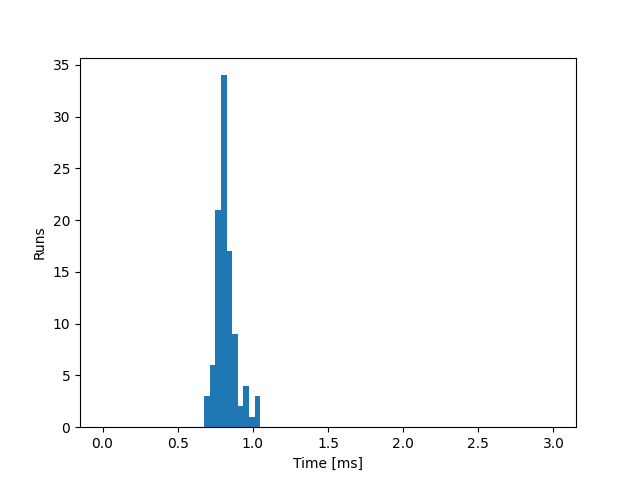
\includegraphics[width=\textwidth]{tests/sorting.native.png}
    \caption{Native}
  \end{subfigure}
  \begin{subfigure}[b]{0.32\textwidth}
    \centering
    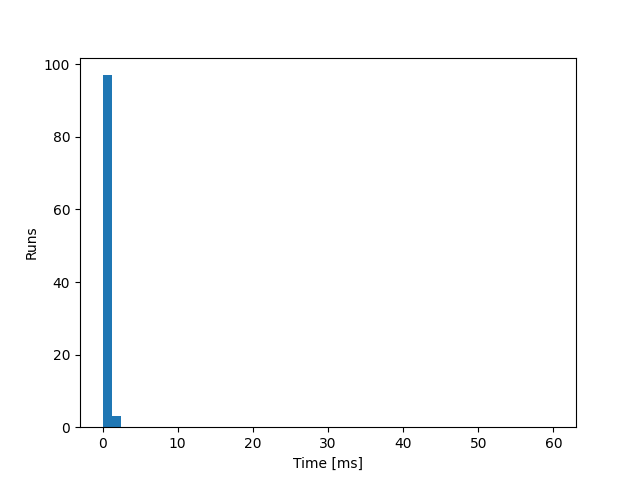
\includegraphics[width=\textwidth]{tests/sorting.native-landlock.png}
    \caption{Landlock}
  \end{subfigure}
  \begin{subfigure}[b]{0.32\textwidth}
    \centering
    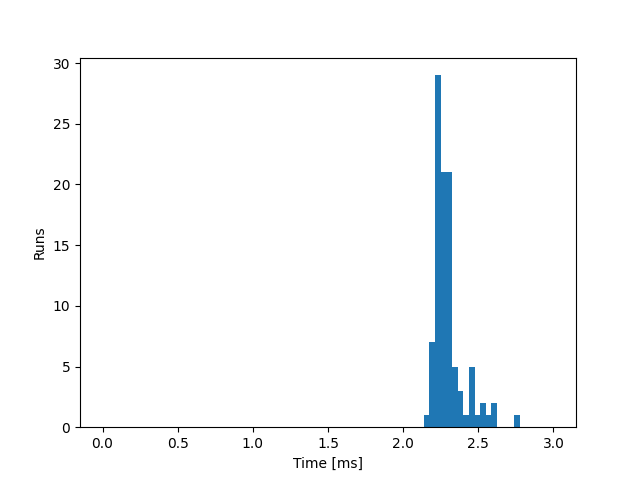
\includegraphics[width=\textwidth]{tests/sorting.native-bpf.png}
    \caption{eBPF}
  \end{subfigure}
  \caption{Distribution of execution times when sorting 10000 numbers (native).}
  \label{fig:distribution-sorting-native}
\end{figure}

\begin{figure}[ht!]
  \centering
  \begin{subfigure}[b]{0.32\textwidth}
    \centering
    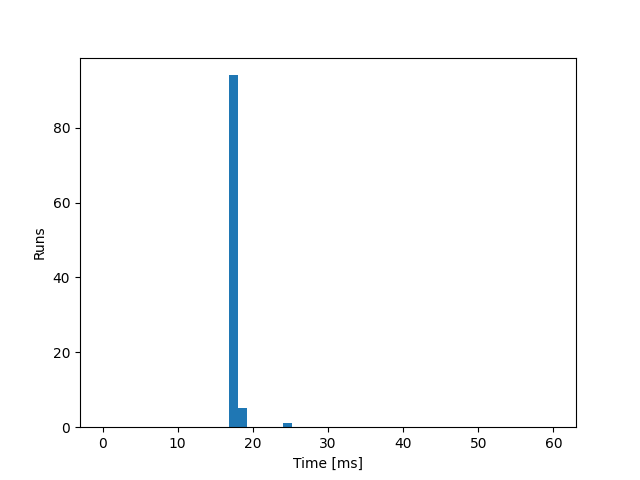
\includegraphics[width=\textwidth]{tests/sorting.wasmtime.png}
    \caption{Wasmtime}
  \end{subfigure}
  \begin{subfigure}[b]{0.32\textwidth}
    \centering
    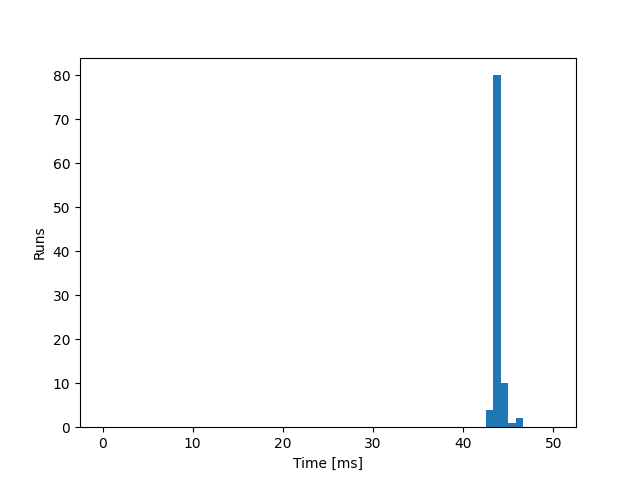
\includegraphics[width=\textwidth]{tests/sorting.wasm-landlock.png}
    \caption{WASM + Landlock}
  \end{subfigure}
  \begin{subfigure}[b]{0.32\textwidth}
    \centering
    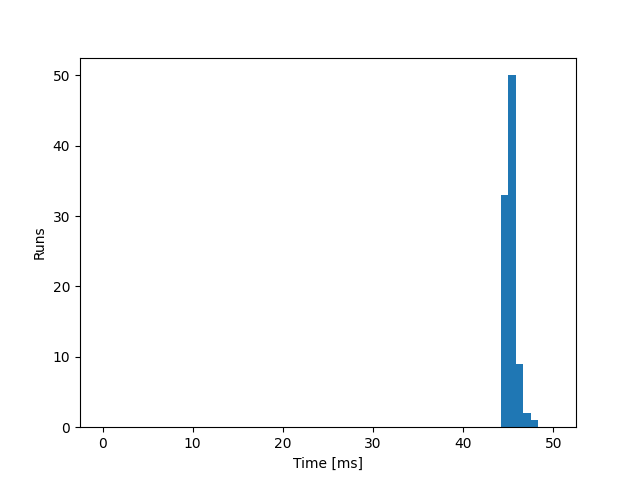
\includegraphics[width=\textwidth]{tests/sorting.wasm-bpf.png}
    \caption{WASM + eBPF}
  \end{subfigure}
  \caption{Distribution of execution times when sorting 10000 numbers (WASM).}
  \label{fig:distribution-sorting-wasm}
\end{figure}

\subsection{Opening a file}

This set of tests is meant to measure how the sandboxes perform when the restricted program opens a file.
In this case, the performance is measured by reading an empty file with the program described in Listing \ref{lst:reading-test-rust}.
For the policy used with eBPF, its outline is highlighted in Listing \ref{lst:outline-policy-reading-test}
- in this case, it is necessary to give permissions to access the terminal since the size of the read content is printed. 

\vspace*{0.5cm}
\begin{code}[language=yaml, caption=The outline of the policy used for testing the reading program., label=lst:outline-policy-reading-test]
name: test-reading-file

cmd: # The command to be executed

allow:
  - device: terminal
  - fs: {pathname: ., access: rxm}
\end{code}

As is visible in Tables \ref{table:lsm-impact-native} and \ref{table:lsm-impact-wasm},
the same considerations made for a purely computational program are valid in this case too
- Landlock, on average, is much closer to native speed than eBPF.
This is also shown in Figure \ref{fig:distribution-opening-native}, where the eBPF curve is shifted towards
higher execution times.

Similarly, the WASM tests present the same behaviour remarked in the previous section -
even when unrestricted, WASM is much slower than a native binary, and the developed runtime
still has the constant overhead of around $30\ ms$ in both the tests within the Landlock and eBPF sandboxes.
Again, Figure \ref{fig:distribution-opening-wasm} shows the distribution of execution times.

\begin{figure}[ht]
  \centering
  \begin{subfigure}[b]{0.32\textwidth}
    \centering
    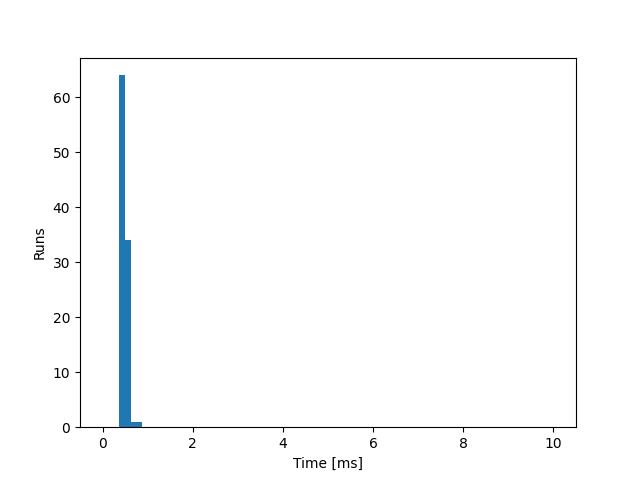
\includegraphics[width=\textwidth]{tests/reading-file-0.native.png}
    \caption{Native}
  \end{subfigure}
  \begin{subfigure}[b]{0.32\textwidth}
    \centering
    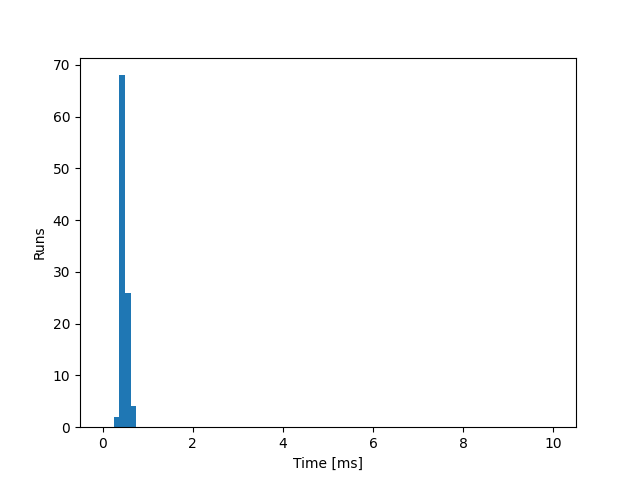
\includegraphics[width=\textwidth]{tests/reading-file-0.native-landlock.png}
    \caption{Landlock}
  \end{subfigure}
  \begin{subfigure}[b]{0.32\textwidth}
    \centering
    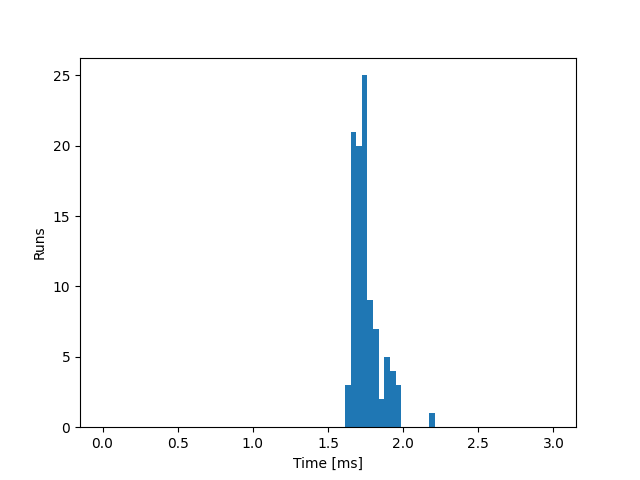
\includegraphics[width=\textwidth]{tests/reading-file-0.native-bpf.png}
    \caption{eBPF}
  \end{subfigure}
  \caption{Distribution of execution times when opening a file (native).}
  \label{fig:distribution-opening-native}
\end{figure}

\begin{figure}[ht]
  \centering
  \begin{subfigure}[b]{0.32\textwidth}
    \centering
    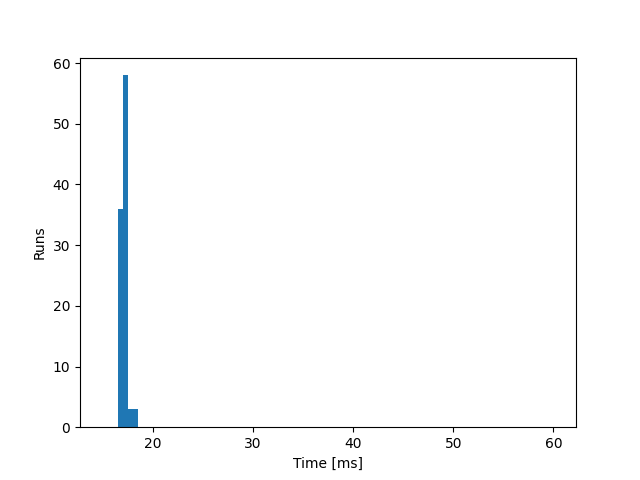
\includegraphics[width=\textwidth]{tests/reading-file-0.wasmtime.png}
    \caption{Wasmtime}
  \end{subfigure}
  \begin{subfigure}[b]{0.32\textwidth}
    \centering
    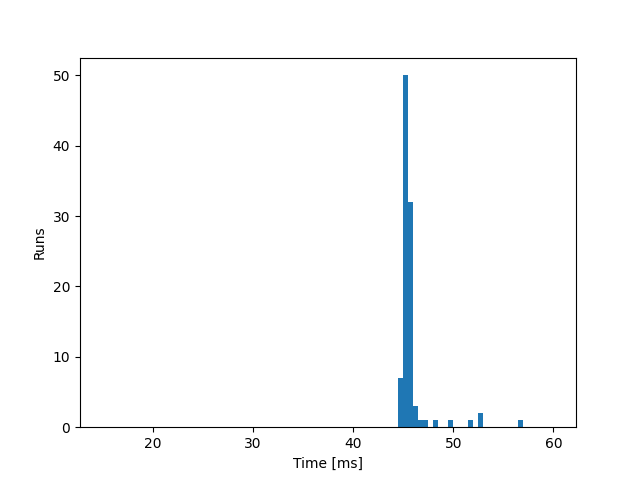
\includegraphics[width=\textwidth]{tests/reading-file-0.wasm-landlock.png}
    \caption{WASM + Landlock}
  \end{subfigure}
  \begin{subfigure}[b]{0.32\textwidth}
    \centering
    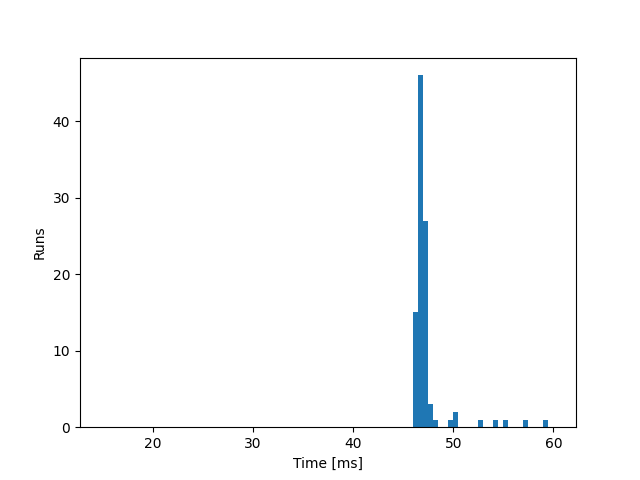
\includegraphics[width=\textwidth]{tests/reading-file-0.wasm-bpf.png}
    \caption{WASM + eBPF}
  \end{subfigure}
  \caption{Distribution of execution times when opening a file (WASM).}
  \label{fig:distribution-opening-wasm}
\end{figure}

\subsection{Accessing the file system}

This last batch of tests is meant to show how sandboxed binaries, both native and WASM, performs when
dealing with progressively large files.
The following figures, namely Figure \ref{fig:avg-comparison-native-speed} and Figure \ref{fig:avg-comparison-wasm-speed},
represents how the average execution time of a native binary and a WASM binary, respectively, changes
when the read file gets bigger.

The first notable feature is that performance drops exponentially as the file gets larger,
starting to drop when reading a file in the order of tens of MBs, and with a significant
spike in execution times when reaching the order of hundreds of MBs.
This slow-down is clearly visible in the native curves as well as in the WASM curves,
hence it has to be independent of the method used to run the
program and only due to external circumstances, such as the operating system or the disk reading speed.
For small files, however, there is not a notable change in speed.

Another point of note is that in Figure \ref{fig:avg-comparison-native-speed} the gap between eBPF and Landlock,
identified in the previous sections, is clearly visible at all file sizes.
This can be seen also in Figure \ref{fig:avg-comparison-wasm-speed}, albeit less clearly as the file reaches $100$ MB.
Note that, while the WASM runtime used for restricting a WASM binary with Landlock is the same used when testing eBPF,
in this last case Landlock was disabled altogether, so any performance difference is only due to eBPF's internals.

Again, the WASM curves in Figure \ref{fig:avg-comparison-wasm-speed} clearly show the overhead
of about $30\ ms$ identified in the previous sections - the \textit{WASM+Landlock} and \textit{WASM+eBPF} curves
exhibit the same trend as the \textit{Wasmtime} one, but appear translated by a constant factor.

\begin{figure}[ht!]
  \centering
  \begin{subfigure}[b]{\textwidth}
    \centering
    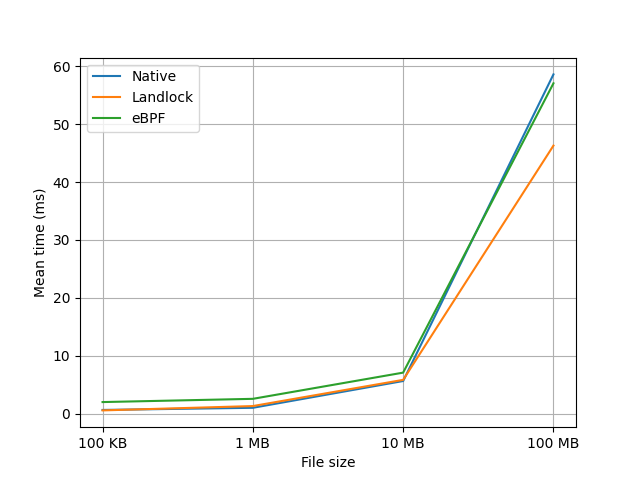
\includegraphics[width=0.8\linewidth]{tests/reading-file-native-graph.png}
  \end{subfigure}

  \begin{subfigure}[b]{0.45\textwidth}
    \centering
    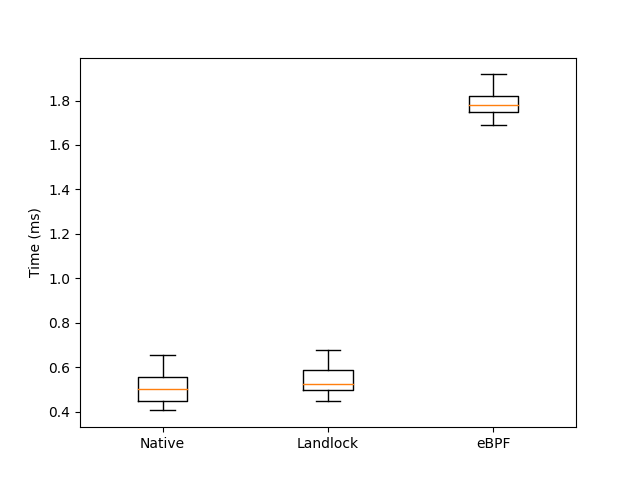
\includegraphics[width=\textwidth]{tests/box-plot-100K.native.png}
    \caption{Box plot for reading a 100 KB file.}
  \end{subfigure}
  \begin{subfigure}[b]{0.45\textwidth}
    \centering
    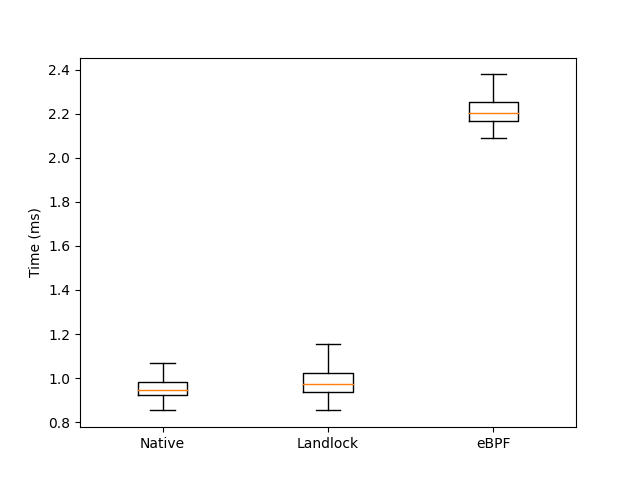
\includegraphics[width=\textwidth]{tests/box-plot-1M.native.png}
    \caption{Box plot for reading a 1 MB file.}
  \end{subfigure}
  \begin{subfigure}[b]{0.45\textwidth}
    \centering
    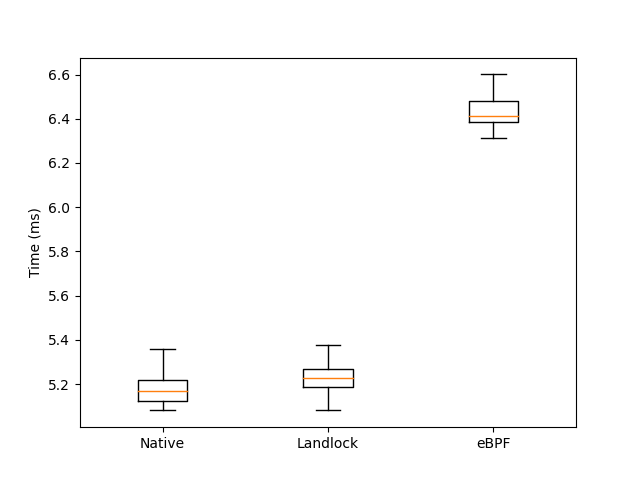
\includegraphics[width=\textwidth]{tests/box-plot-10M.native.png}
    \caption{Box plot for reading a 10 mB file.}
  \end{subfigure}
  \begin{subfigure}[b]{0.45\textwidth}
    \centering
    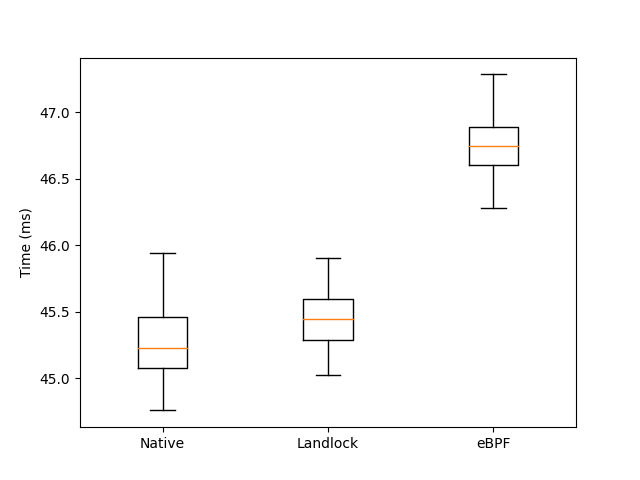
\includegraphics[width=\textwidth]{tests/box-plot-100M.native.png}
    \caption{Box plot for reading a 100 MB file.}
  \end{subfigure}

  \caption{A comparison of native average speeds when reading a file.}
  \label{fig:avg-comparison-native-speed}
\end{figure}

\begin{figure}[ht!]
  \centering
  \begin{subfigure}[b]{\textwidth}
    \centering
    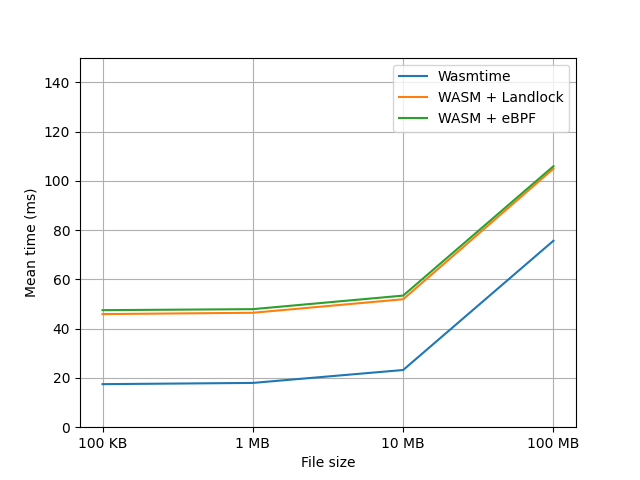
\includegraphics[width=0.8\linewidth]{tests/reading-file-wasm-graph.png}
  \end{subfigure}

  \begin{subfigure}[b]{0.45\textwidth}
    \centering
    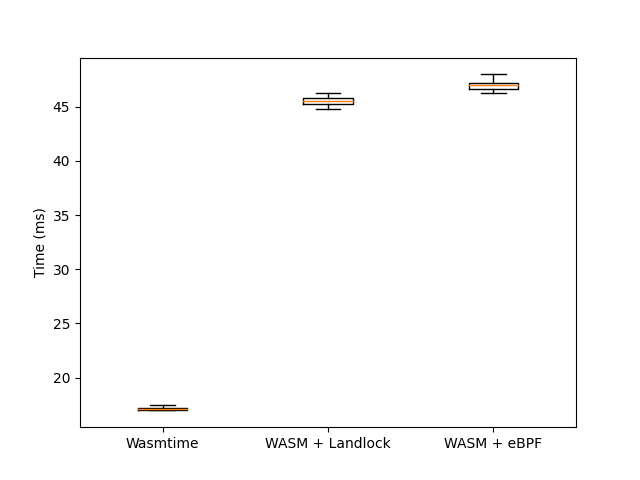
\includegraphics[width=\textwidth]{tests/box-plot-100K.wasm.png}
    \caption{Box plot for reading a 100 KB file.}
  \end{subfigure}
  \begin{subfigure}[b]{0.45\textwidth}
    \centering
    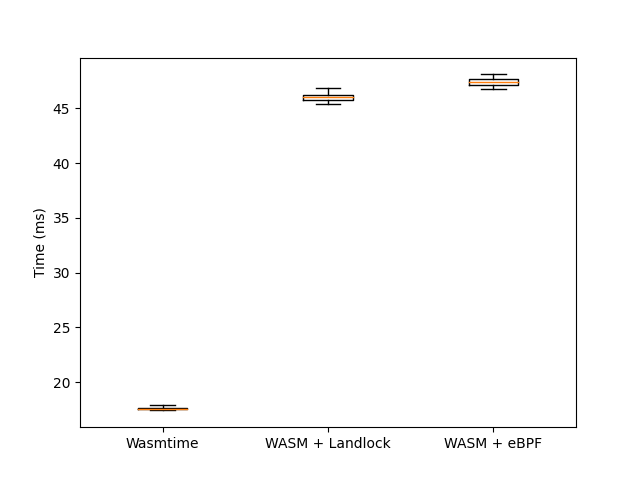
\includegraphics[width=\textwidth]{tests/box-plot-1M.wasm.png}
    \caption{Box plot for reading a 1 MB file.}
  \end{subfigure}
  \begin{subfigure}[b]{0.45\textwidth}
    \centering
    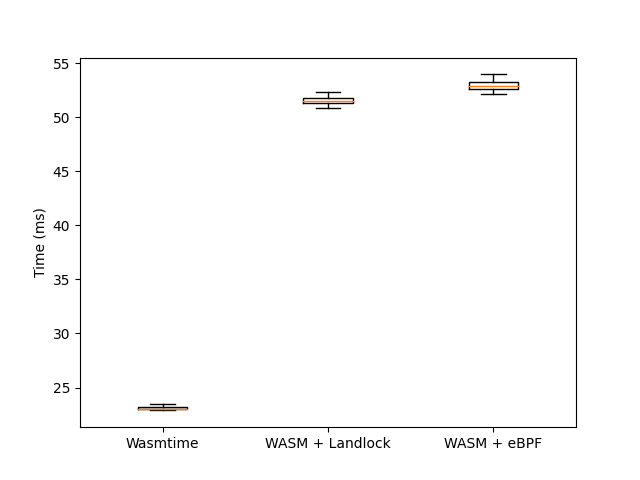
\includegraphics[width=\textwidth]{tests/box-plot-10M.wasm.png}
    \caption{Box plot for reading a 10 mB file.}
  \end{subfigure}
  \begin{subfigure}[b]{0.45\textwidth}
    \centering
    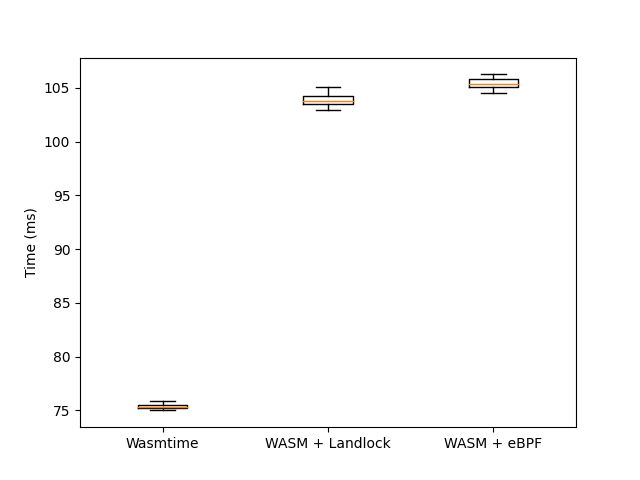
\includegraphics[width=\textwidth]{tests/box-plot-100M.wasm.png}
    \caption{Box plot for reading a 100 MB file.}
  \end{subfigure}

  \caption{A comparison of WASM average speeds when reading a file.}
  \label{fig:avg-comparison-wasm-speed}
\end{figure}

\clearpage
Finally, Figure \ref{fig:distribution-reading-native} and Figure \ref{fig:distribution-reading-wasm}
collect all distribution relative to the different readings for native binaries and WASM binaries, respectively.
Note that, in both figures, the tests on the $100$ MB file have a different scale from the others.

\begin{figure}[ht!]
  \centering
  \begin{subfigure}[b]{0.32\textwidth}
    \centering
    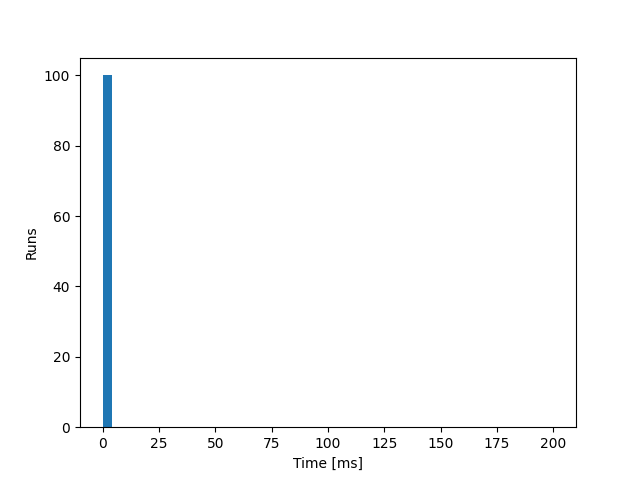
\includegraphics[width=\textwidth]{tests/reading-file-100k.native.png}
    \caption{Native (100 KB)}
  \end{subfigure}
  \begin{subfigure}[b]{0.32\textwidth}
    \centering
    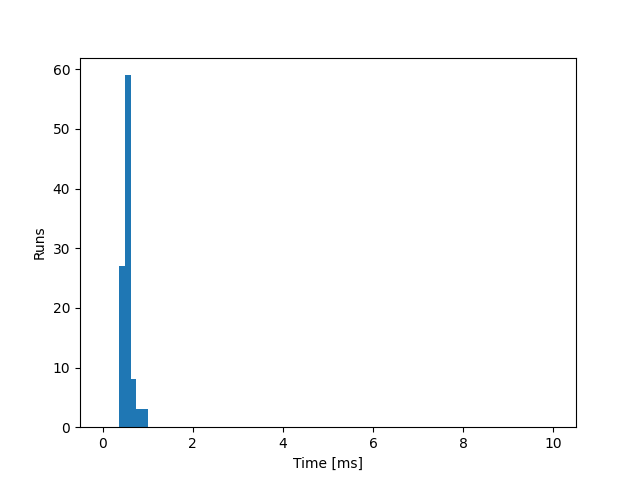
\includegraphics[width=\textwidth]{tests/reading-file-100k.native-landlock.png}
    \caption{Landlock (100 KB)}
  \end{subfigure}
  \begin{subfigure}[b]{0.32\textwidth}
    \centering
    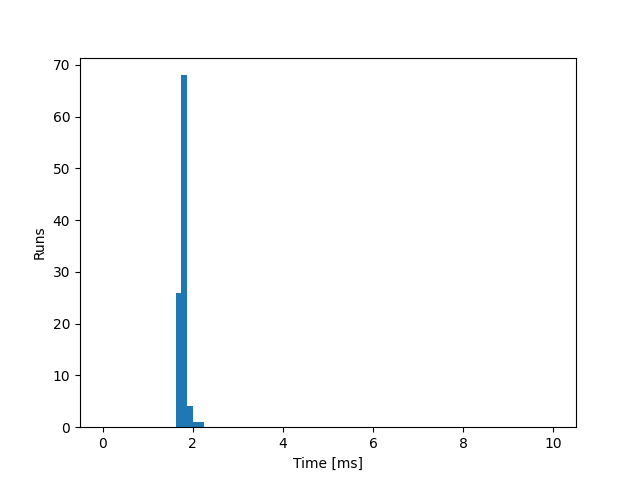
\includegraphics[width=\textwidth]{tests/reading-file-100k.native-bpf.png}
    \caption{eBPF (100 KB)}
  \end{subfigure}

  \begin{subfigure}[b]{0.32\textwidth}
    \centering
    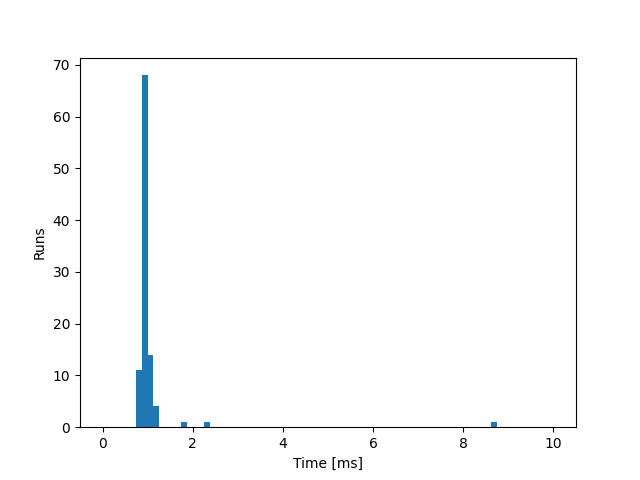
\includegraphics[width=\textwidth]{tests/reading-file-1M.native.png}
    \caption{Native (1 MB)}
  \end{subfigure}
  \begin{subfigure}[b]{0.32\textwidth}
    \centering
    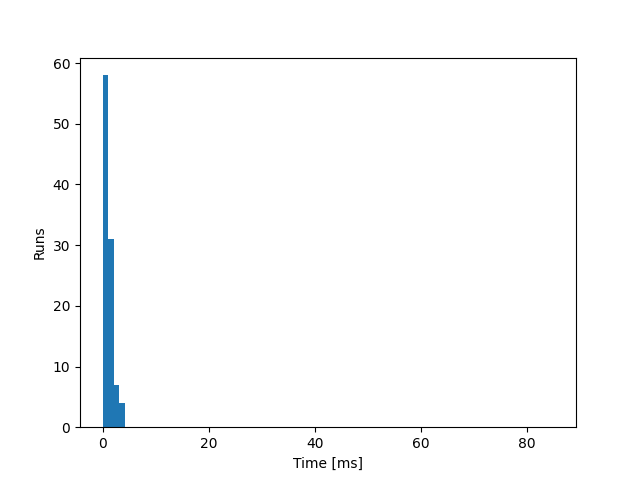
\includegraphics[width=\textwidth]{tests/reading-file-1M.native-landlock.png}
    \caption{Landlock (1 MB)}
  \end{subfigure}
  \begin{subfigure}[b]{0.32\textwidth}
    \centering
    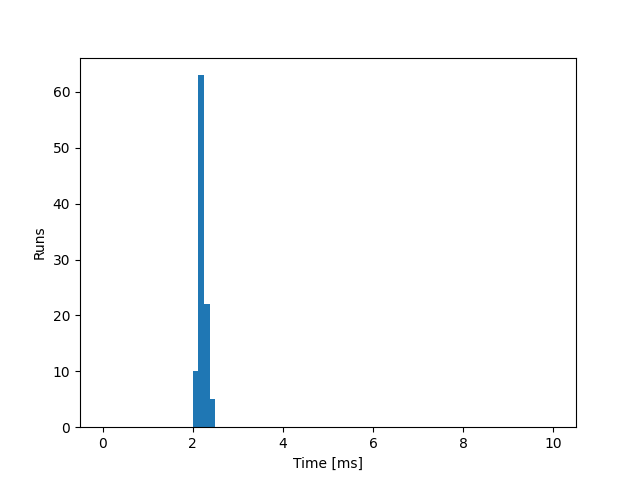
\includegraphics[width=\textwidth]{tests/reading-file-1M.native-bpf.png}
    \caption{eBPF (1 MB)}
  \end{subfigure}

  \begin{subfigure}[b]{0.32\textwidth}
    \centering
    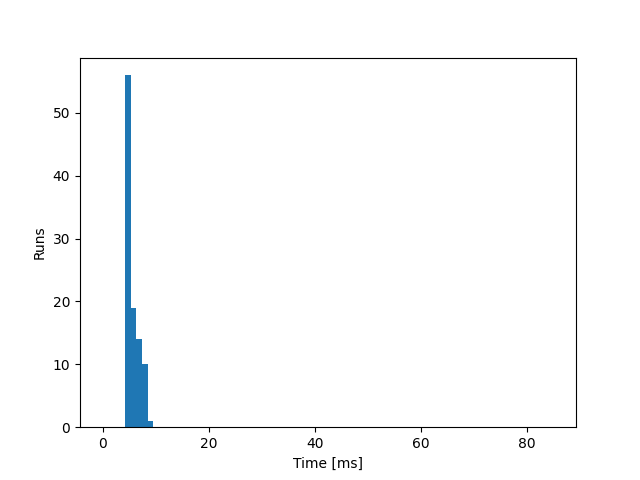
\includegraphics[width=\textwidth]{tests/reading-file-10M.native.png}
    \caption{Native (10 MB)}
  \end{subfigure}
  \begin{subfigure}[b]{0.32\textwidth}
    \centering
    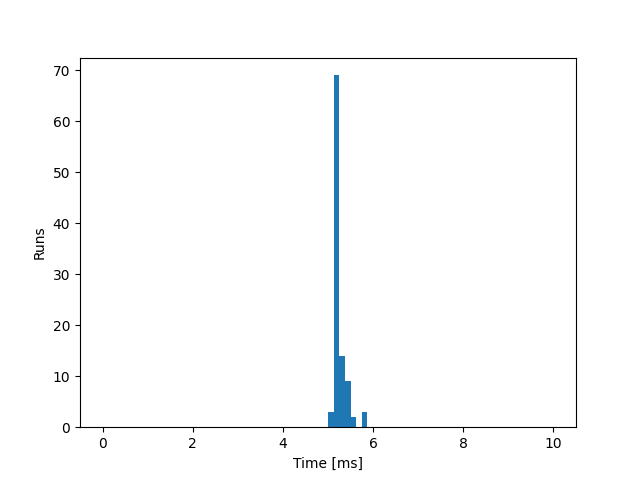
\includegraphics[width=\textwidth]{tests/reading-file-10M.native-landlock.png}
    \caption{Landlock (10 MB)}
  \end{subfigure}
  \begin{subfigure}[b]{0.32\textwidth}
    \centering
    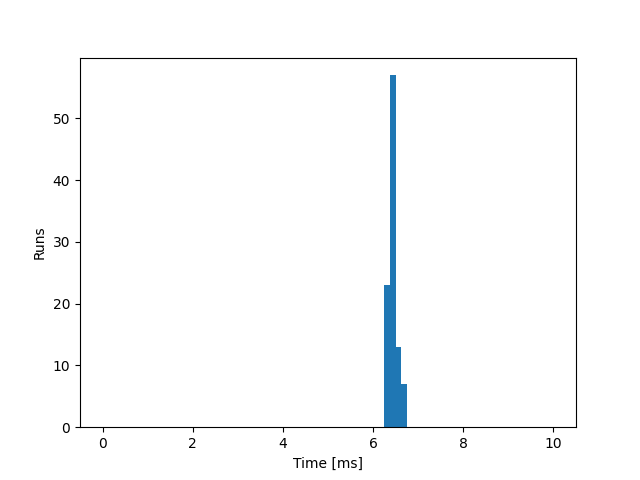
\includegraphics[width=\textwidth]{tests/reading-file-10M.native-bpf.png}
    \caption{eBPF (10 MB)}
  \end{subfigure}

  \begin{subfigure}[b]{0.32\textwidth}
    \centering
    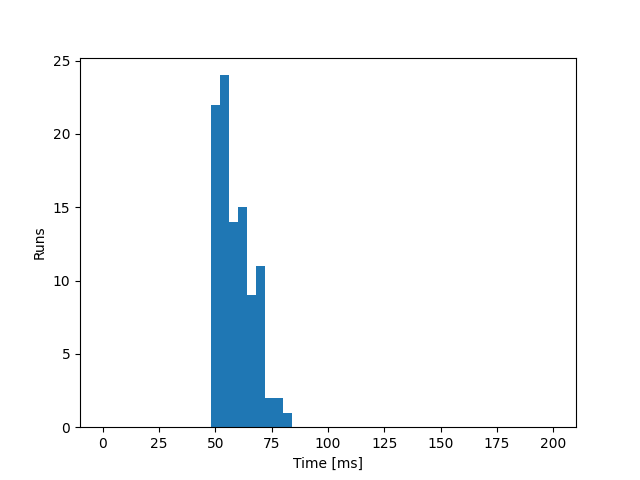
\includegraphics[width=\textwidth]{tests/reading-file-100M.native.png}
    \caption{Native (100 MB)}
  \end{subfigure}
  \begin{subfigure}[b]{0.32\textwidth}
    \centering
    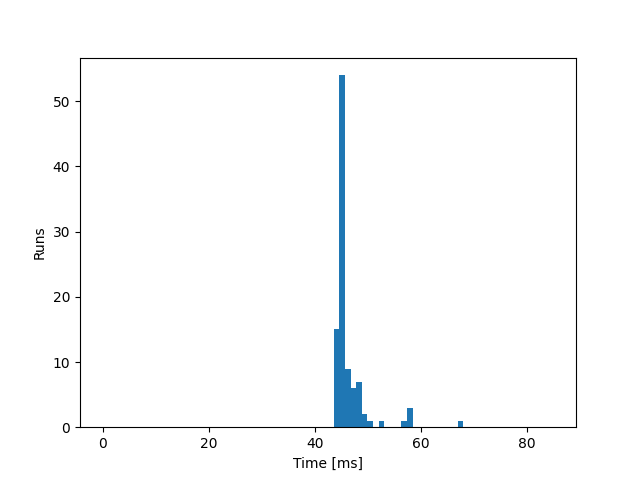
\includegraphics[width=\textwidth]{tests/reading-file-100M.native-landlock.png}
    \caption{Landlock (100 MB)}
  \end{subfigure}
  \begin{subfigure}[b]{0.32\textwidth}
    \centering
    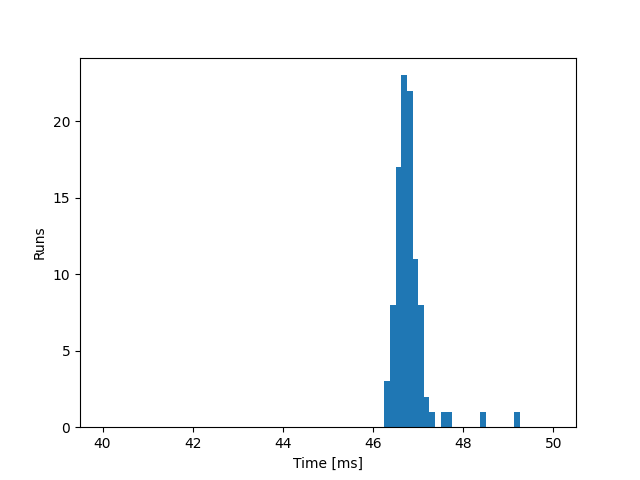
\includegraphics[width=\textwidth]{tests/reading-file-100M.native-bpf.png}
    \caption{eBPF (100 MB)}
  \end{subfigure}

  \caption{Distribution of a native binary execution times when reading a file.}
  \label{fig:distribution-reading-native}
\end{figure}

\begin{figure}[ht!]
  \centering
  \begin{subfigure}[b]{0.32\textwidth}
    \centering
    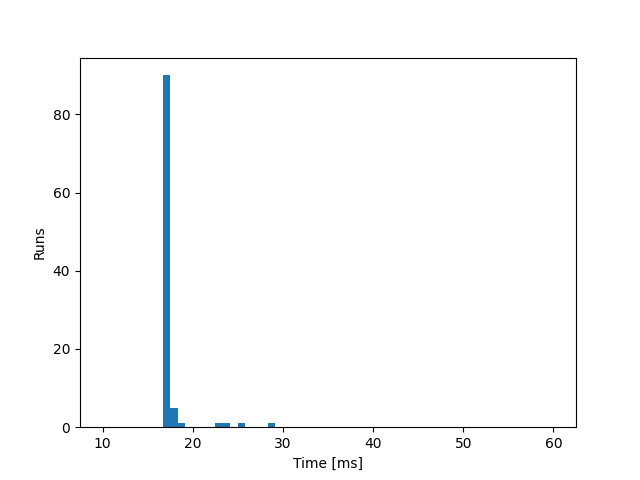
\includegraphics[width=\textwidth]{tests/reading-file-100k.wasmtime.png}
    \caption{Wasmtime (100 KB)}
  \end{subfigure}
  \begin{subfigure}[b]{0.32\textwidth}
    \centering
    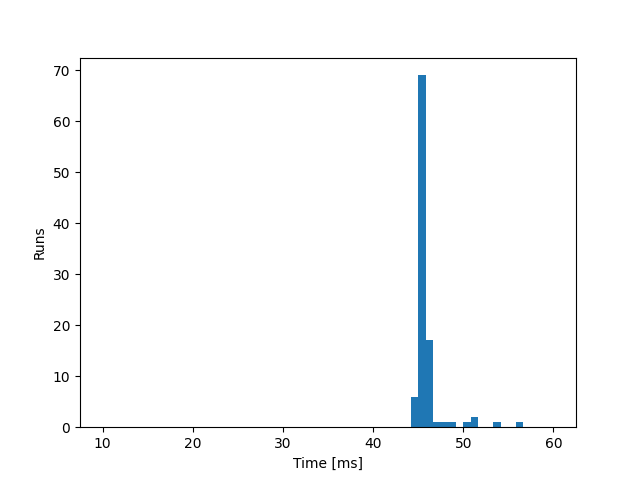
\includegraphics[width=\textwidth]{tests/reading-file-100k.wasm-landlock.png}
    \caption{Landlock (100 KB)}
  \end{subfigure}
  \begin{subfigure}[b]{0.32\textwidth}
    \centering
    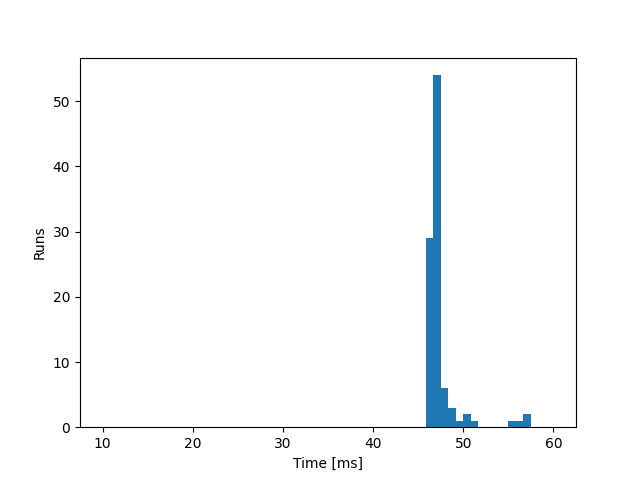
\includegraphics[width=\textwidth]{tests/reading-file-100k.wasm-bpf.png}
    \caption{eBPF (100 KB)}
  \end{subfigure}

  \begin{subfigure}[b]{0.32\textwidth}
    \centering
    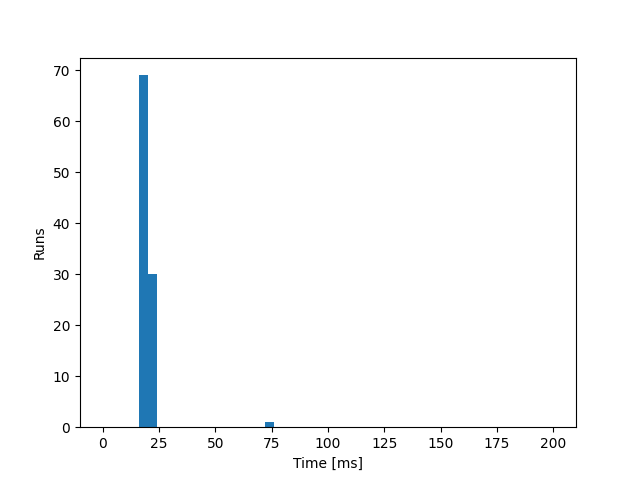
\includegraphics[width=\textwidth]{tests/reading-file-1M.wasmtime.png}
    \caption{Wasmtime (1 MB)}
  \end{subfigure}
  \begin{subfigure}[b]{0.32\textwidth}
    \centering
    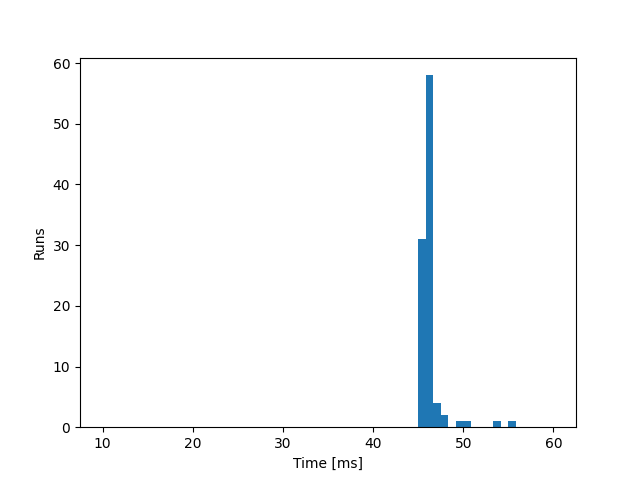
\includegraphics[width=\textwidth]{tests/reading-file-1M.wasm-landlock.png}
    \caption{Landlock (1 MB)}
  \end{subfigure}
  \begin{subfigure}[b]{0.32\textwidth}
    \centering
    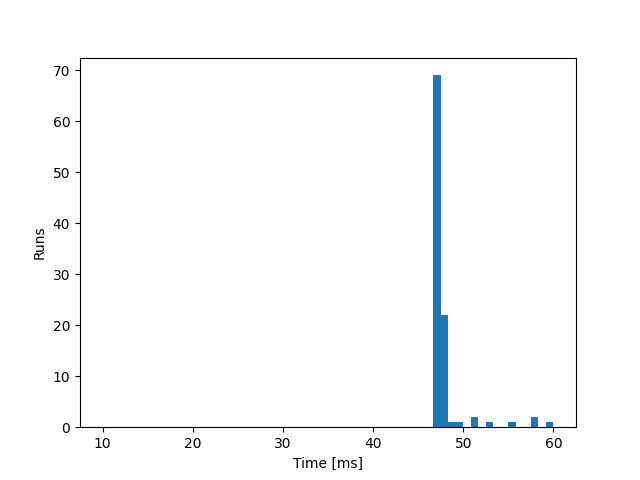
\includegraphics[width=\textwidth]{tests/reading-file-1M.wasm-bpf.png}
    \caption{eBPF (1 MB)}
  \end{subfigure}

  \begin{subfigure}[b]{0.32\textwidth}
    \centering
    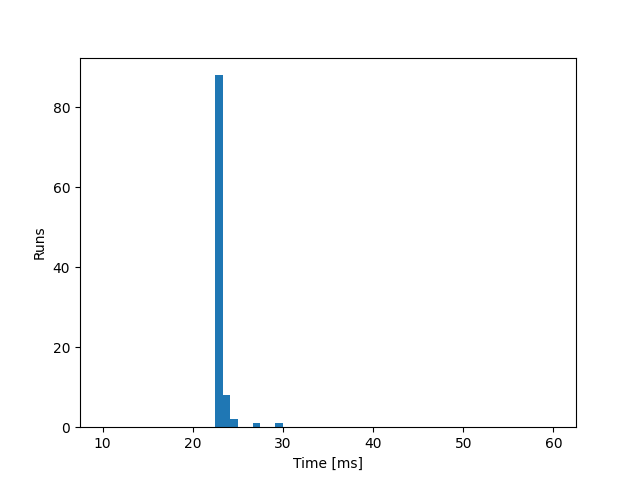
\includegraphics[width=\textwidth]{tests/reading-file-10M.wasmtime.png}
    \caption{Wasmtime (10 MB)}
  \end{subfigure}
  \begin{subfigure}[b]{0.32\textwidth}
    \centering
    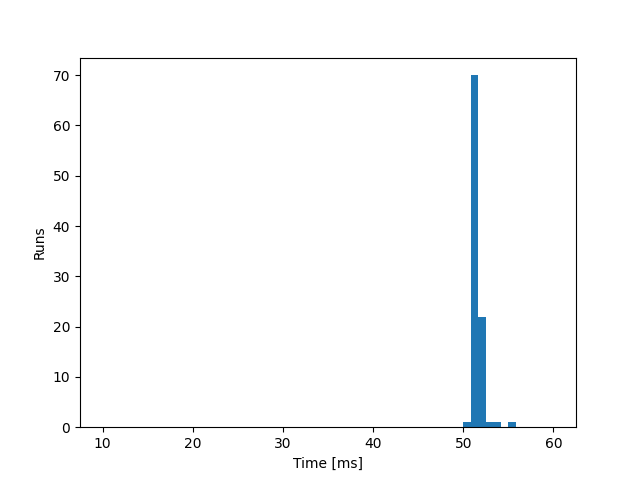
\includegraphics[width=\textwidth]{tests/reading-file-10M.wasm-landlock.png}
    \caption{Landlock (10 MB)}
  \end{subfigure}
  \begin{subfigure}[b]{0.32\textwidth}
    \centering
    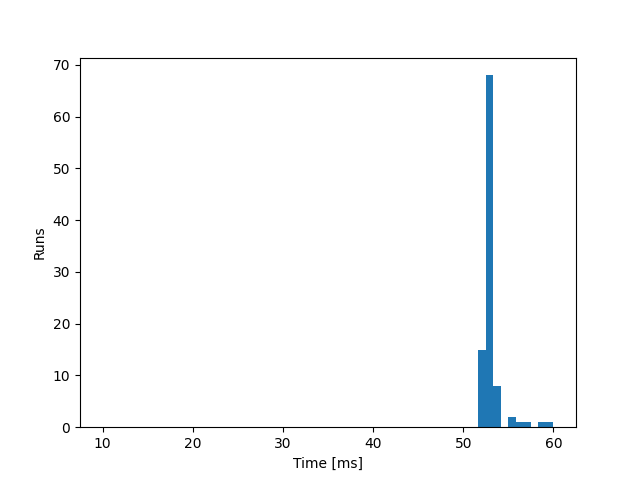
\includegraphics[width=\textwidth]{tests/reading-file-10M.wasm-bpf.png}
    \caption{eBPF (10 MB)}
  \end{subfigure}

  \begin{subfigure}[b]{0.32\textwidth}
    \centering
    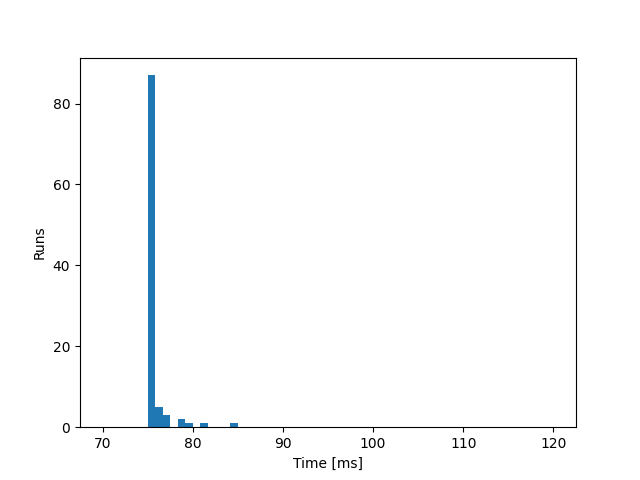
\includegraphics[width=\textwidth]{tests/reading-file-100M.wasmtime.png}
    \caption{Wasmtime (100 MB)}
  \end{subfigure}
  \begin{subfigure}[b]{0.32\textwidth}
    \centering
    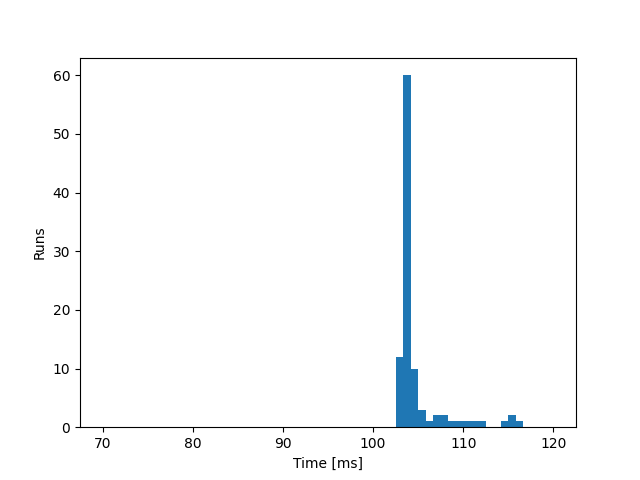
\includegraphics[width=\textwidth]{tests/reading-file-100M.wasm-landlock.png}
    \caption{Landlock (100 MB)}
  \end{subfigure}
  \begin{subfigure}[b]{0.32\textwidth}
    \centering
    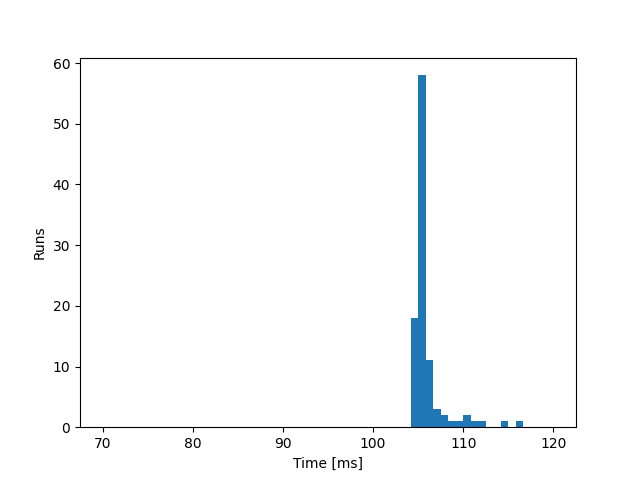
\includegraphics[width=\textwidth]{tests/reading-file-100M.wasm-bpf.png}
    \caption{eBPF (100 MB)}
  \end{subfigure}

  \caption{Distribution of a WASM binary execution times when reading a file.}
  \label{fig:distribution-reading-wasm}
\end{figure}

\clearpage

\section{Internal analysis of the developed project}
\label{sec:performance-internal-analysis}

The goal of this series of tests is to measure how the developed runtime,
described in Section \ref{sec:restricting-wasi-landlock}, behaves internally.
To do this, various timestamps were taken and combined in specific parts of the
code in order to have some data on the execution time of important program parts,
which are
\begin{itemize}
  \item command line argument parsing;
  \item WASM module instantiation;
  \item the preopening of all directories by the Wasmtime library;
  \item collecting and applying all the Landlock rules;
  \item and finally, compiling and running the WASM module.
\end{itemize}

Note that this project only considers Landlock and not eBPF, since eBPF is enforced externally
by a different process, while Landlock system calls are embedded in the code of the runtime.
Hence, only the impact of Landlock can be measured \textit{internally} in the code.

\vspace*{0.5cm}

\begin{code}[language=Rust, caption=The tested trivial program, label=lst:project-perf-program-simple]
fn main() {
  println!("Hello World");
}
\end{code}

\begin{code}[language=Rust, caption=The more complex tested program, label=lst:project-perf-program-complex]
use std::fs::{read_to_string, write};

fn main() -> {
  read_to_string("file1.txt").expect("Read error");
  write("file1.txt", "Content 1").expect("Write error");
  read_to_string("file2.txt").expect("Read error");
  write("file2.txt", "Content 2").expect("Write error");
}  
\end{code}

\begin{table}[ht!]
  \centering
  \csvreader[
    tabular={|l|r|r|r|r|},
    table head = \hline
      \textit{Program part} & $\mu_I$ & $\sigma_I$ & $\mu_C$ & $\sigma_C$   \\ \hline\hline,
    late after line = \\ \hline,
    head to column names,
  ]{test-data/project-stats-simple.csv}{}
  {\type & \mean & \stddev & \meanc & \stddevc}
  \caption{Execution times in $ms$ when running the simple program (Listing \ref{lst:project-perf-program-simple}).}
  \label{table:execution-times-simple}
\end{table}

\begin{table}[ht!]
  \centering
  \csvreader[
    tabular={|l|r|r|r|r|},
    table head = \hline
      \textit{Program part} & $\mu_I$ & $\sigma_I$ & $\mu_C$ & $\sigma_C$   \\ \hline\hline,
    late after line = \\ \hline,
    head to column names,
  ]{test-data/project-stats-medium.csv}{}
  {\type & \mean & \stddev & \meanc & \stddevc}
  \caption{Execution times in $ms$ when running the complex program (Listing \ref{lst:project-perf-program-complex}).}
  \label{table:execution-times-complex}
\end{table}

\subsection{Execution times}
\label{sec:performance-internal-analysis-execution-times}

The various measures are taken by using the standard Rust library \texttt{std::time},
in particular the \texttt{Instant} struct, and then averaged on a total of 100 runs of
two particular programs:
\begin{itemize}
  \item a trivial one visible in Listing \ref{lst:project-perf-program-simple},
        dealing only with printing a simple string to the terminal;
  \item a more complex one visible in Listing \ref{lst:project-perf-program-complex},
        reading and writing some files, so that specific Landlock permissions are required
        (specifically, reading and writing files).
\end{itemize}

Tables \ref{table:execution-times-simple} and \ref{table:execution-times-complex} contains
all measured data in milliseconds for, respectively, the trivial and complex program.
The visible timestamps are both the average time spent by a section, given by $\mu_I$,
and the cumulative time up until that section's completion, given by $\mu_C$.
Standard deviations $\sigma_I$ and $\sigma_C$ are also given for any respective program part.
For example, if the part ``Landlock enforcement'' is such that $\mu_I = 20$ and $\mu_C = 100$,
this means that on average it takes $20\ ms$ to apply Landlock to the running process, and on average this part
is fully completed after $100\ ms$ from the beginning of the program.

Moreover, Figure \ref{fig:perf-execution-times-comparison} shows how each program section
occupies the overall time spent running by the program. The various labels are as follows
- \texttt{A} is for ``Argument parsing'', \texttt{B} is for ``Module initialisation'',
\texttt{C} is for ``Preopen'', \texttt{D} is for ``Landlock enforcement'' and
\texttt{E} is for ``Running WASM binary''.

\begin{figure}[ht!]
  \centering
  
  \begin{subfigure}[b]{0.46\textwidth}
    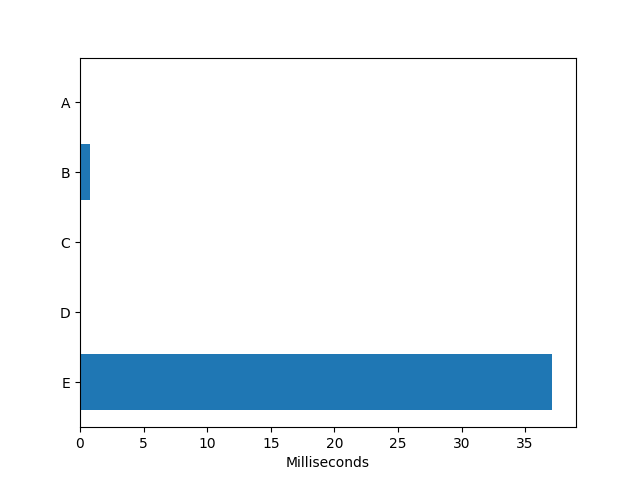
\includegraphics[width=\textwidth]{project-performance/graph_simple.png}
    \caption{Simple program}
  \end{subfigure}
  \begin{subfigure}[b]{0.46\textwidth}
    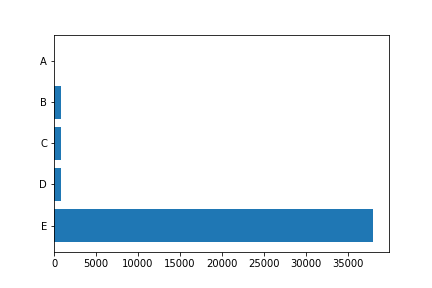
\includegraphics[width=\textwidth]{project-performance/graph_simple_c.png}
    \caption{Simple program (cumulative)}
  \end{subfigure}

  \begin{subfigure}[b]{0.46\textwidth}
    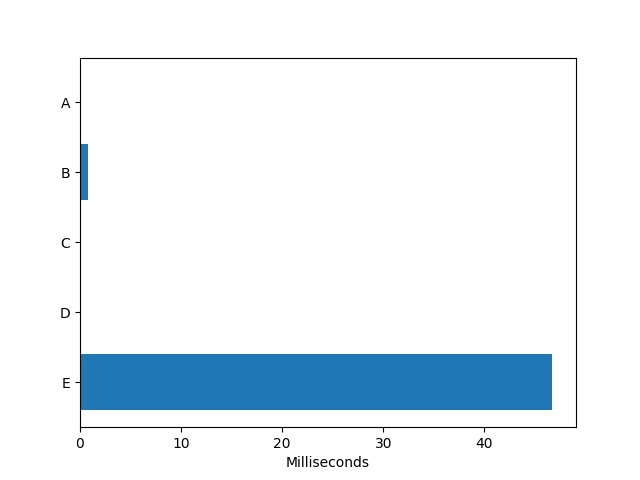
\includegraphics[width=\textwidth]{project-performance/graph_medium.png}
    \caption{Complex program}
  \end{subfigure}
  \begin{subfigure}[b]{0.46\textwidth}
    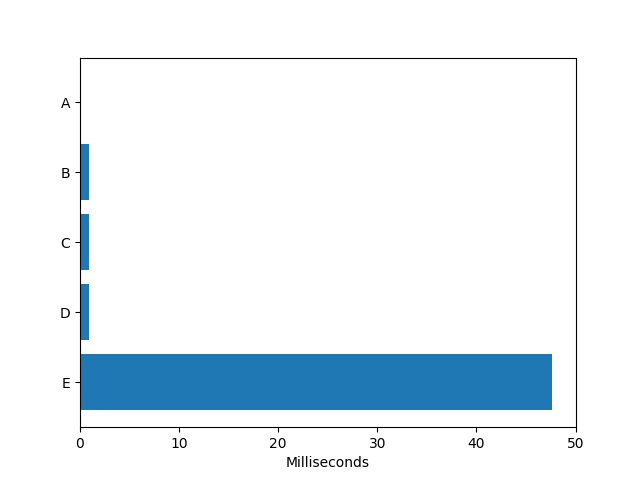
\includegraphics[width=\textwidth]{project-performance/graph_medium_c.png}
    \caption{Complex program (cumulative)}
  \end{subfigure}

  \caption{A graphic comparison of all the execution times.}
  \label{fig:perf-execution-times-comparison}
\end{figure}

As is immediately apparent by the collected data, the biggest bottleneck on performance is given
by \textit{running the WebAssembly} binary with the library provided by Wasmtime.
The specific actions required are instantiating the required structures, interpreting and linking the WASM module,
and finally running it, as already highlighted in Section \ref{sec:landlock-wasm-module}.
This section alone makes up $97.7 \%$ of the time spent running the trivial program, and $98.1 \%$ of the time
spent running the complex program.

The next biggest chunk of time is spent into \textit{module initialisation}, which is comprised of the
reading of the WASM binary file into memory and the instantiation of specific context structures used
to keep track of preopened directories. For both programs, this is around $800\ \mu s$ in duration.

On the other hand, enforcing Landlock does not have a substantial impact on performance,
and it is even faster than the argument parsing algorithm.

This findings further support the data shown in Section \ref{sec:performance-comparison-between-different-sandboxes} -
it was found that the developed WASM runtime was much slower than calling \textit{Wasmtime} from the command
line, but because Landlock had little overhead when dealing with native binaries this implied that
the ``culprit'' for the constant overhead could be the \textit{Wasmtime} library.
In this case, it can also be seen than the time took for running the WASM binary is, in both cases, about
the same as the constant overhead that appeared when restricting WASM binaries through the developed runtime.

\section{Conclusions and observations}

One of the key points of this series of tests is that, although perfectly usable,
WebAssembly is not still at the level of performance provided by using a native binary.
As seen in Section \ref{sec:performance-comparison-between-different-sandboxes}, WASM binaries
always perform worse than the native counterpart, even when not restricted by a LSM.
This result is however to be expected - a WASM binary is made up of WASM instructions and
it is similar to a sort of \textit{bytecode} that is interpreted by the runtime of one's choosing,
and usually a interpreted program\footnote{Although the program in question is a binary format and hence faster to interpret.}
is slower than a compiled one.
This is true also for other languages that follow this paradigm - for example, Java with the JVM
or Python (that can be compiled into a bytecode before being interpreted) are usually regarded as
slower and/or more resource-hungry when compared to compiled languages such as C or Rust.

When embedding WebAssembly in another language, this performance gap becomes even higher due to
the work that must be done through the provided interpreting libraries
(see Section \ref{sec:performance-internal-analysis-execution-times}).

A positive point that has been shown multiple times, however, is that restricting a binary
with a LSM, be it Landlock or eBPF, does not worsen performance a lot.
As seen in Section \ref{sec:performance-comparison-between-different-sandboxes}, although a small
performance impact is present, this could be considered negligible for large programs that take
some time to run. For small programs that have an execution time of the same order of magnitude
as the delay introduced this could become however problematic if they are called multiple time
and in high frequency.